
\section{Evaluation}
\label{sec:evaluation}
We evaluate the performance of {\specula} using Amazon's EC2. We deployed the system over geo-distributed datacenters and evaluated with three workloads: a synthetic workload, TPC-C and RUBiS. We compare two variations of our protocol, one that only performs speculative read ({\specula}-Internal) and one that can perform both speculative read and speculative commit ({\specula}-External), with two state-of-the-art protocols. The results show that even without externalizing speculative results, we can achieve about 3.5$\times$ speedup for workloads with high local contention and low remote contention. Nevertheless, allowing speculative commit can further reduce latency by XXX. \textbf{How to write latency reduction? For some workload, our final latency is 300 while the baselin is 21000, so we say by a factor or 70? What about for perceived latency?}

\subsection{Protocol variations and baselines}
We include two variations of our protocol, {\specula}-Internal and  {\specula}-External. As their name suggests, {\specula}-Internal only allows speculative read, thus it only internally does speculation; on the other hand, {\specula}-External allows both speculative read and speculative commit, thus it can externalize speculative results to users. We run both of these protocols with an automatic tuning process. The automatic tuning process collects throughput statistics from all machines every twenty seconds \textbf{should I mention that?}, determines the next speculation level and then informs all servers. With the automatic-tuner, {\specula}-Internal can only enable or disable speculative read, while {\specula}-External starts with having no speculative read (No SR), then enabling speculative read (SR) until enabling speculative read with speculation length eight (SR+SL8). 

We compare our protocol against two baseline protocols. The first one is based on ClockSI \cite{clocksi}, a decentralized transactional protocol that provides Snapshot Isolation. The original ClockSI protocol does not support replication and we added a simple replication mechanism: when a master partition receives a prepare request, it synchronously replicates it to its replicas. The replicas then acknowledge to the transaction coordinator directly and the coordinator commits the transaction when it has received prepare from all involved partitions and their replicas. The protocol requires one and half WAN round-trip to commit a transaction. We name it as \textbf{ClockSI-Rep}.

The second baseline is designed to emulate PLANET \cite{pang2014planet}, which permits speculatively committing transaction while not allowing speculative read or pipelining speculative transactions.  The originally proposed PLANET is built on top of the MDCC protocol \cite{kraska2013mdcc} and decides to speculative commit a transaction or not by a prediction model. Since it is not possible to do an apple-to-apple comparison, we emulate a simplified version of PLANET, by building it atop ClockSI-Rep and additionally allows each client to speculatively commit one transaction. 

\subsection{Experimental setup}
\label{subsec:setup}
We implemented our baseline protocol and speculative protocol using the Erlang programming language, on top of \textit{antidote}, an open-source reference platform for evaluating distributed consistency protocols \cite{antidote}.

We deployed the system in nine datacenters of Amazon EC2: Ireland(IE), Seoul(SU), Sydney(SY), Oregon(OR), Singapore(SG), North California(CA), Frankfurt(FR), Tokyo(TY) and North Virginia(VA). Each datacenter consists of three m4.large instances (2 VCPU and 8 GB of memory) and each instance holds the master replica of one partition. All DCs form a consistent hashing ring according to the order of the above list; the data of each instance is replicated by five following datacenters' corresponding servers, e.g. the data of DC CA is replicated by DCs FR, TY, VA, IE and SU. We interleave DCs from nearby regions in the hash ring, so that different replication group will have similar latency to perform replication , as shown in table \ref{tab:latency}.

We locate a workload stressor in each instance that issues transactions to local transaction coordinators. If a transaction is aborted, the client retries it until it gets committed. Therefore, the final latency of an operation is calculated as its commit time minus its first start time (as it may have been tried a few times), while perceived latency is the last time it was report as speculative commit minus its first start time.

Each experiment is run for three times. We discard the aggregate results of the first twenty seconds and show the average value (deviation is low).

\begin{table*}
\small
\begin{center}
  \begin{tabular}{l |  l | l | l| l | l | l| l| l |l } 
     & IE & SU& SY& OR & SG & CA &  FR & TY & VA  \\ \hline
  \textbf{Max latency (replicas)} & 334(SG) & 267(FR) & 321(FR) & 160(SG)  & 337(IE) & 167(FR) & 321(SY)& 212(IE)  &  226(SY)  \\   \hline
  \textbf{Max latency (all)} &  334(SG) &  267(FR) & 321(FR)  & 163(SY) & 337(IE) & 175(SG) & 324(SG)  & 233(FR)  & 226(SY) \\ \hline
  \end{tabular}
\end{center}
\caption{Maximal mean latency of a DC to its replicas and to all other DC}
\label{tab:latency}
\end{table*}


\subsection{Synthetic workloads}
Our evaluation starts with synthetic workloads. The synthetic workloads simulate idealistic non-interactive workloads, where each thread issues a new transaction as soon as the previous one is committed (or speculative committed). The tunable speculation levels are the following, from conservative to aggressive: no speculative read (SR for short) and speculation length zero (SL0), SR and SL0, SR and SL1, ..., SR and SL8. We first compare {\specula}-Strong and {\specula}-Tuning with the baselines, then via a separate experiment we compare the effectiveness of auto-tuning method with static configurations.

\paragraph{Transaction and data access} A transaction reads 10 keys then updates them. 90\% of key access goes to a small range of each data partition, a.k.a hotspot, and we adjust the size of hotspot to control contention rate. Each data partition has two million keys, of which one million are only accessible by local-initiated transactions and the other are only accessible by remote transactions. This allows adjusting local contention level (i.e. the contention level when a local transaction performs local certification) without affecting remote conflict level. In the following experiments, we denote 30000 keys for the size of local hotspot size as \textbf{low local contention} and 1000 keys as \textbf{high local contention}; according, 15000 keys for a remote hotspot is named \textbf{low remote contention} and 500 for \textbf{high remote contention}. The following workloads use high data locality: 80\% access goes to local master partitions, while 20\% goes to slave data partitions replicated locally.

\begin{figure*}
\centering
\def\svgwidth{0.98\columnwidth}
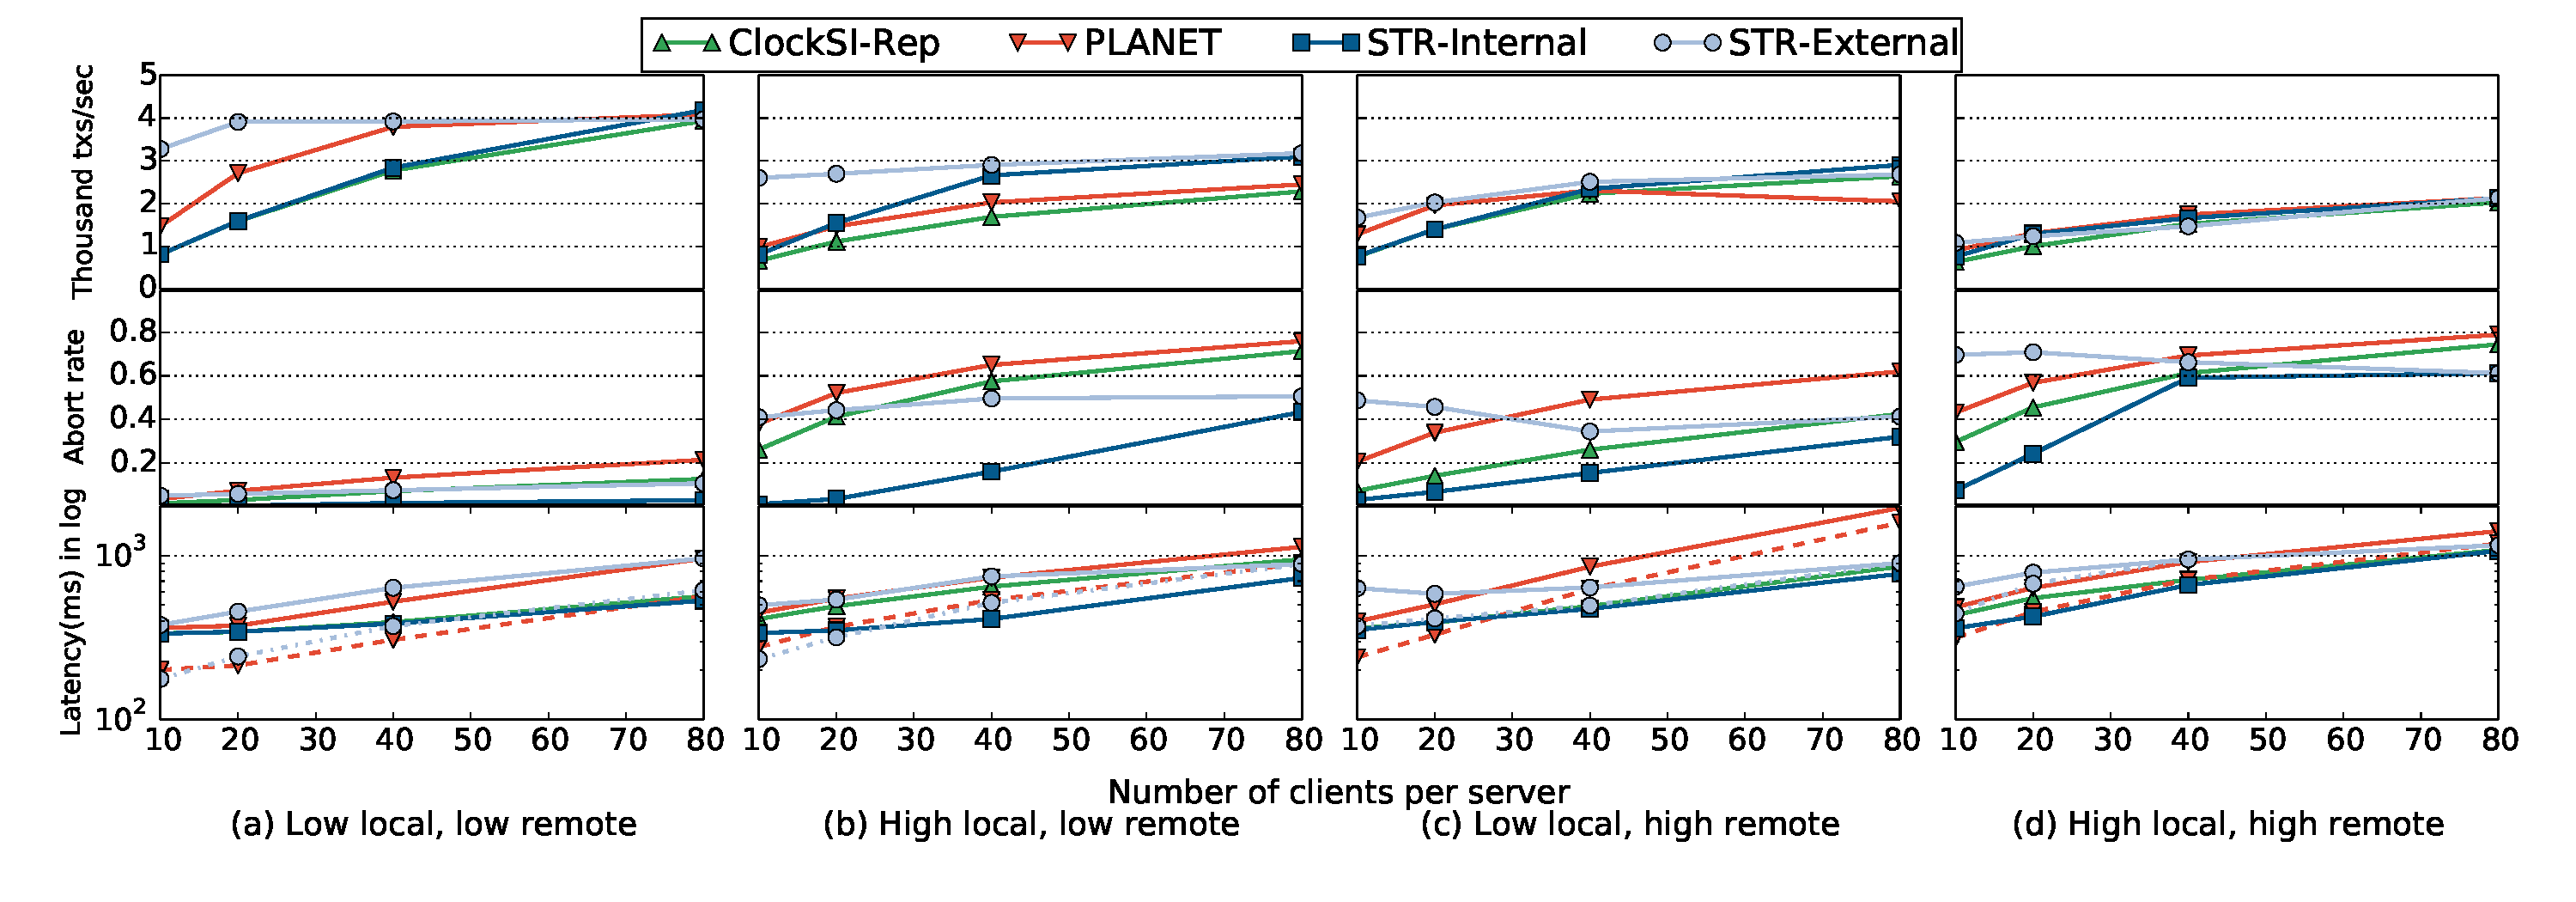
\includegraphics[scale=0.35]{figures/micro}
\hspace{-10mm}
\caption{\textit{Performance of different protocols under four levels of contention.} \textit{Low local, low remote} denotes low local contention and low remote contention, and so forth. For latency, solid lines denote operation's latency and dashed lines denote the user perceived latency.}
\label{fig:micro_conflict}
\end{figure*}


\begin{figure}[t]
\centering
\def\svgwidth{0.98\columnwidth}
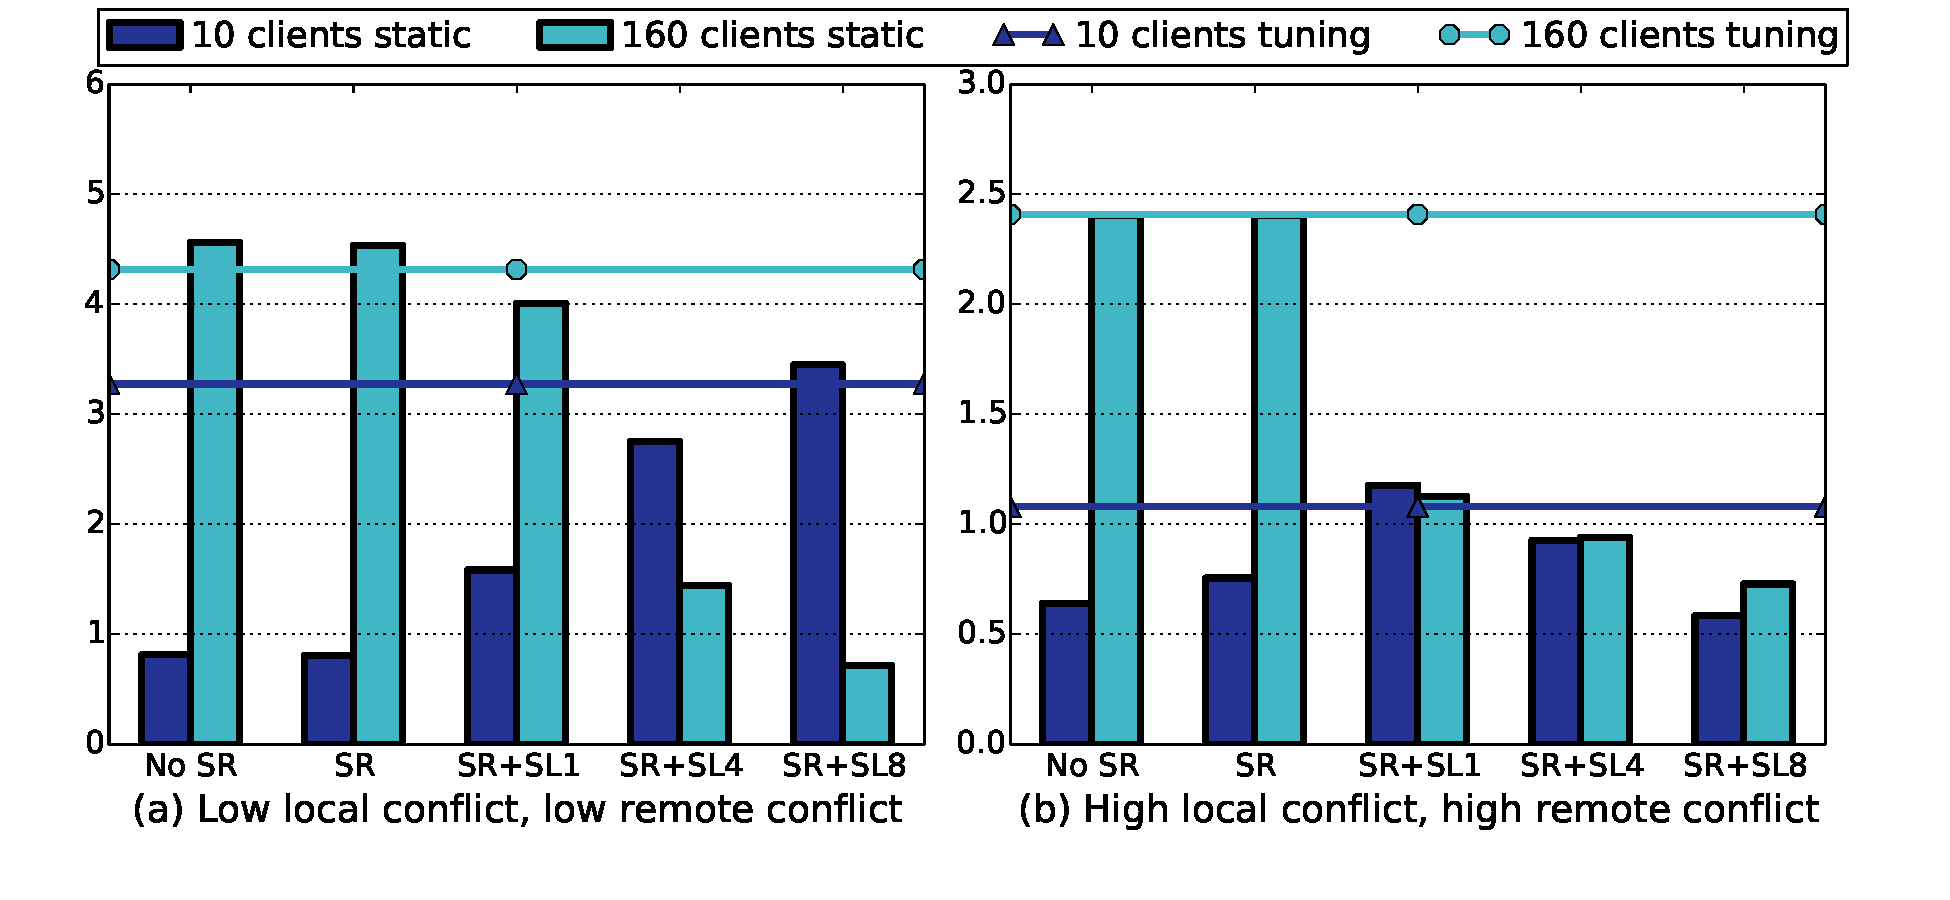
\includegraphics[scale = 0.28]{figures/tuning}
\vspace{-7mm}
\caption{\footnotesize The throughput of tuning versus static configuration}
\label{fig:tuning}
\end{figure}

\paragraph{Performance under different contentions} In this set of experiments, we vary contention levels and system load, i.e. number of clients, to examine the performance of ClockSI-Rep, PLANET, {\specula}-Internal and {\specula}-External. As mentioned, both variations of {\specula} are equipped with automatic tuning methods. 

For low contention workload (\ref{fig:micro}a), both PLANET and {\specula}-External achieve good speedup, because they all allow speculatively committing transactions so clients can perform more work. Though, the key difference is that {\specula}-External supports pipelining multiple transactions, so it can achieve high throughput with much fewer clients than PLANET. The speedup reduces when the system gets more saturated. {\specula}-Internal has very little speedup, as this workload has low contention so speculative read rarely occurs. Still, {\specula}-Internal has much lower conflict rate than both ClockSI-Rep and PLANET due to the use of PreciseClock.

Figure \ref{fig:micro}b shows the throughput of different protocols in a workload with high local contention and low remote contention. This workload is beneficial for {\specula}-Internal and {\specula}-External, as they allow speculative read to avoid getting blocked when trying to read pre-commit records, and transactions being speculatively-read are likely to commit due to low remote contention. On the other hand, because PLANET does permit not speculative read, it achieves littler performance gain. The effect of speculative read is directly reflected in latency: the latency of PLANET and ClockSI-Rep considerably increase compared with figure \ref{fig:tuning}a, while the latency of {\specula}-Internal and {\specula}-External are not affected due to speculative read.

Next, we examine workloads with high remote contention, which is unfavorable for speculation. As figure \ref{fig:micro}c shows, PLANET has large performance penalty and large latency, as speculative commit often fails due to high remote contention. Although {\specula}-Strong also allows speculative commit, thanks to the auto-tuning algorithm, it get good throughput despite the number of clients. The performance of STR-Internal are similar to ClockSI-Rep again (as in figure \ref{fig:micro}), due to having low local contention. The last workload combines both high local contention and high remote contention, but {\specula}-External and {\specula}-Internal still remain stable throughput due to auto-tuning. Nevertheless, PLANET achieves higher throughput than in figure \ref{fig:micro}c, because high local contention causes transactions to be blocked and perform less speculative commit.

\paragraph{Automatic tuning v.s. static configurations} This experiment compares the throughput of 10 clients and 160 clients per server, using either automatic tuning or static tuning, e.g. not allowing speculative read (No SR), allowing speculative read and speculative commit with length one (SR+SL1). We picked two extreme workloads, one with low local and remote contention, and one with high contention for both. As shown in figure \ref{fig:tuning}, the levels of speculation to achieve optimal throughput vary for different numbers of clients and different contention, which is hard to predict in advance. This is indeed what we observed when experimenting different speculation levels and motivated us to design the automatic tuning method. More importantly, as can be seen in the figure, the curve of speculation level to throughput is convex, i.e. if a speculation level gives local maximal throughput, this is guaranteed to be a global maximum throughput. This observation drove us to design the automatic tuning method as a simple hill climbing algorithm \cite{hillclimbing}, which is simple and fast yet can reach throughput close to the optimal throughput (figure \ref{fig:tuning}).


%Reading a key that is not replicated locally causes large latency, which makes it difficult to examine the benefit of speculation. So for most of the experiments, a transaction only accesses keys replicated in local datacenter. We dedicate a separate experiment to examine the effect of remote read on throughput.

\subsection{Macro benchmark}
In the following experiments, we evaluate the performance of \specula with realistic interactive workloads, namely TPC-C\cite{tpcc} and RUBiS \cite{rubis}. The dramatic difference between these workloads and the synthetic ones are, to model realistic human-machine interaction, these workloads specify large 'think time' between consecutive operations issued by a user, from a few seconds to tens of seconds. Therefore, we load the system with larger number of threads per server, in order to saturate the system.

\subsubsection{TPC-C}
TPC-C \cite{tpcc} models the workload of an online shopping system. We implemented three TPC-C transactions, namely payment, new-order and order-status, according to the specification. Payment transaction has very high local contention and low remote contention; new-order transaction has medium level local and remote contention, and order-status is a read-only transaction. According to the described workload mix rule in the specification, we come up with three workloads: 5\% new-order, 83\% payment and 12\% order-status (TPC-C A); 5\% new-order, 43\% payment and 52\% order-status (TPC-C B) and 45\% new-order, 43\% payment and 12\% order-status (TPC-C C). We add the 'think time' and 'key time' for each transaction as described in the specification, so a client sleeps for some time (from 5 seconds to as large as hundreds of seconds) both before and after issuing a transaction. In the following experiments, we load each server with five warehouses.

Figure \ref{fig:tpcc}a, \ref{fig:tpcc}b and \ref{fig:tpcc}c show the throughput, latency of update transactions (in logarithm) and abort rate of ClockSI-Rep, PLANET, {\specula}-External and {\specula}-Internal. In general, due to having large think time, speculative commit hardly bring any throughput benefit, while speculative read is important due to these workloads all have high local contention. As a result, PLANET achieves the same throughput as ClockSI-Rep, {\specula}-External achieves the same throughput as {\specula}-Internal, and there is a clear throughput difference between STR and the baselines. Though, with low number of clients, for all three workloads PLANET reduces the perceived latency from about 320 millisecond to about 10 millisecond, a factor of 32. But when the load increases, the local contention is exacerbated and the latency of PLANET also increases. On the other hand, due to allowing speculative read, {\specula}-External and {\specula-Internal} achieve significant speedup compared with the baseline: 2.93$\times$ for TPC-C A, 1.68$\times$ for TPC-C B and 3.47$\times$ for TPC-C C. The latency of both {\specula} protocols also greatly reduce the operation latency by a factor of about 70 of both PLANET and ClockSI-Rep.

\subsection{RUBiS}
RUBiS \cite{rubis} models an online bidding system. Of all the 26 user interactions, there are five update transactions: store bid, store buy now, store comment, register item and register user. RUBiS is designed to run on top of a SQL database, so we did the following modification to adapt it to our key-value store: (i) we horizontally partitioning database tables across servers, so that each server contains an equal portion of data of each table; (ii) many RUBiS insertion operations need to increment a table index to get unique id, which is very inefficient when the table is sharded across machines. To avoid this, we create a local table index for each data shard, as studied in \cite{cecchet2008middleware}. We use RUBiS's 15\% update default workload and its default think time (different transactions can have think time from 2 seconds to 10 seconds).

Due to memory limit, we were not able to load the system with more clients. Nevertheless, the figure still shows that \specula achieves good speedup and latency reduction. With 5000 clients, \specula still achieves about 1.43$\times$ speedup compared with ClockSI-Rep and PLANET. Though, ClockSI-Rep and PLANET, STR-Internal and STR-External achieves similar throughput, due to large think time. Besides, it can be noted that the abort rate of PLANET/ClockSI-Rep even decreases with increasing number of clients. This is because in RUBiS, the access pattern of a client highly depends on the update of other clients, so with more number of clients, the access pattern gets more diverse and the abort rate is reduced.


\begin{figure*}
\centering
\begin{minipage}{.72\textwidth}
\centering
  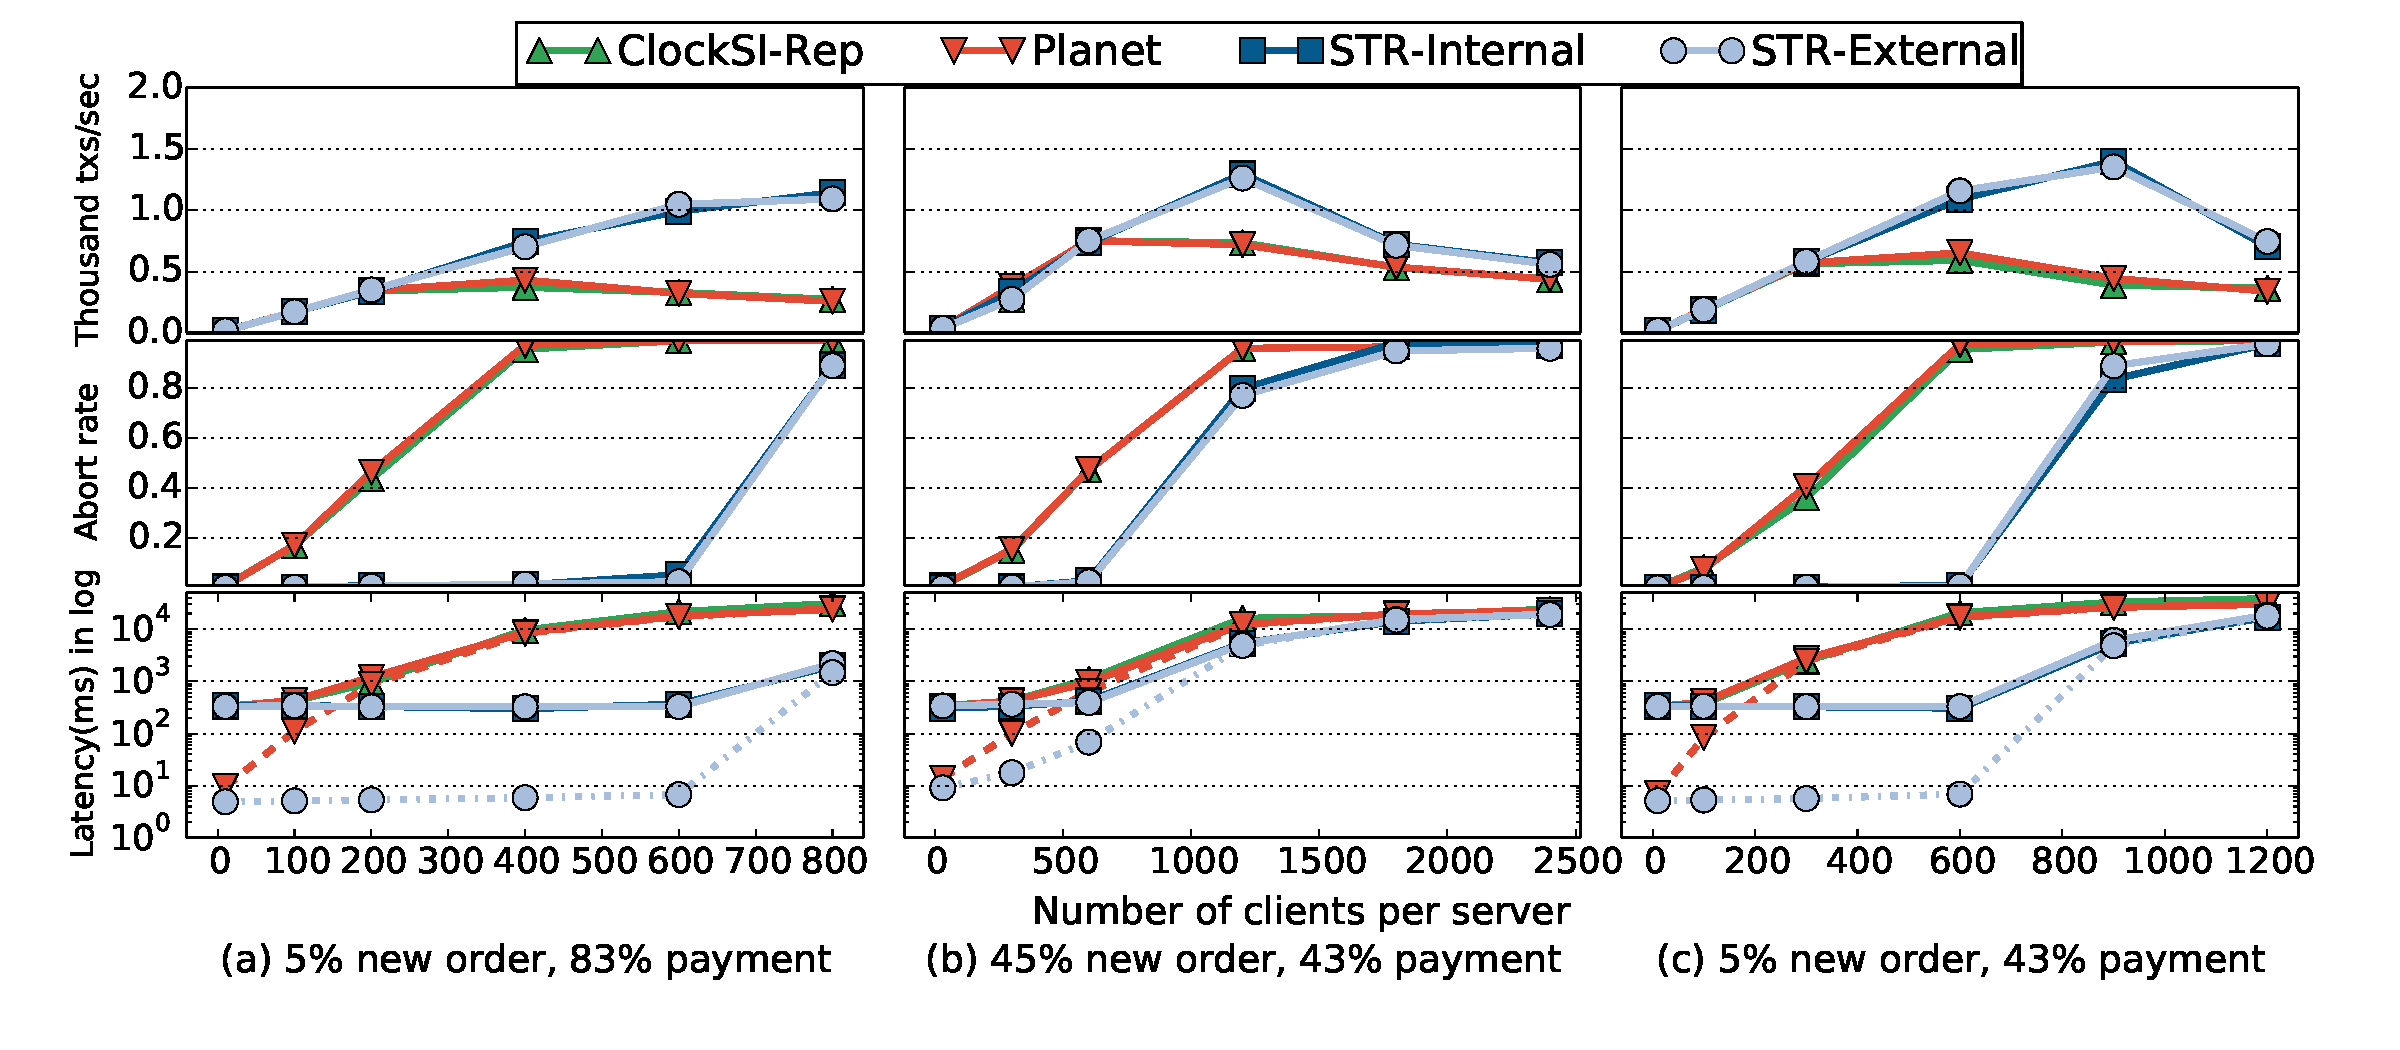
\includegraphics[scale=0.3]{figures/tpcc}
  \vspace{-5mm}
  \caption{The performance of different protocols for three TPC-C workloads.}
  \label{fig:tpcc}
\end{minipage}
\begin{minipage}{.26\textwidth}
\centering
  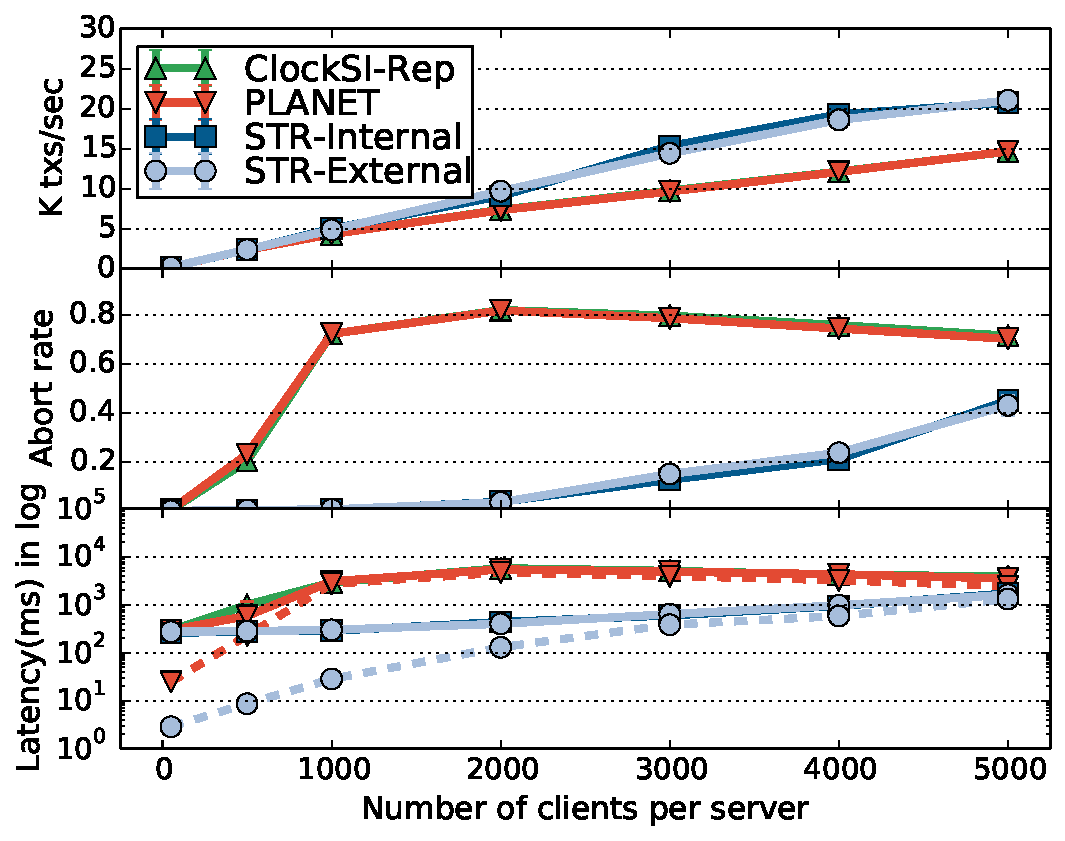
\includegraphics[scale=0.28]{figures/rubislatencywarehouse}
  \vspace{-2mm}
  \caption{The performance of different protocols for RUBiS}
  \label{fig:rubis}
\end{minipage}
\end{figure*}

